\documentclass{article}

\usepackage{amsmath}
\usepackage{amssymb}
\usepackage{listings} % Required for inserting code snippets
\usepackage{xcolor} % Required for inserting colored text
\usepackage{url} % Required for inserting urls
\usepackage{graphicx} % Required for inserting images
\usepackage{subfigure} % Required for inserting subimages
\usepackage{tikz-uml}
\usepackage{graphicx}
\usepackage{float}  % For using [H] specifier
\usepackage{comment} % For multi line comments
\usepackage{subfig}
\usepackage{array} % For table centering 

\sloppy % For making URLs wrap around better
\newcolumntype{P}[1]{>{\centering\arraybackslash}p{#1}} % Centered paragraph table column

\title{Numerical Methods for Partial Differential Equations report}
\author{Mohammadhossein Allahakbari, Michele Miotti, \\Francesco Pesce}
\date{February 1 2024}

\begin{document}

\maketitle

\section{Introduction}
	The Navier-Stokes equations are a set of partial differential equations that describe the motion of viscous fluids. They are named after Claude-Louis Navier and George Gabriel Stokes, who independently developed the equations in the 19th century. The equations are used to model turbulence, which is important in many engineering applications.

This report will focus on the unsteady, incompressible Navier-Stokes equations in two and three dimensions. More specifically, we will consider the "flow past a cylinder" problem, which is a classic benchmark problem in computational fluid dynamics. The problem consists of a fluid flowing past a cylinder, which is placed in a channel. We will start with a brief description of the code structure, followed by a discussion on the mathematical background, with an analysis of the methods used and their convergence and stability properties. We will then present the results for the simulation of the fluid and discuss briefly the implemented preconditioners and their performance and parallel scaling.

All the implemented code is available at \url{https://github.com/FrancescoPesce/nmpde-project3-Allahakbari-Miotti-Pesce} and has been delivered making a pull request to \url{https://github.com/michelebucelli/nmpde-projects}. The code is written in C++ and uses the deal.II library, with the exception of some scripts in Python or Bash. The code was tested using Ubuntu 22.04 as an operating system and requires the set of mk modules for scientific computing. The code is parallelized using MPI and can be compiled using CMake.

\section{Code structure}
	Instructions on how to compile and run the project are available in the \texttt{README.md} file in the root of the repository. A brief description of the code structure and implemented functionalities will be presented.

\subsection{Folder structure}
The root directory of the repository contains the following folders:
\begin{itemize}
    \item \texttt{gmsh} contains the \texttt{.geo} files required for \texttt{gmsh} to generate meshes that describe the problem. These files consists in a list of instructions for \texttt{gmsh} to generate the mesh, such as the size the domain, the shape of the domain, the tag of the boundary conditions, etc.
    
    \item \texttt{include} contains the header files for the C++ code, containing declarations of functions and classes, definitions of template functions and type aliases. Most of the comments regarding the functionalities of the code are in the header files.
    
    \item \texttt{scripts} contains shell scripts for generating meshes with different factors or as standalone files and a simple Python script for generating a plot of the drag and lift coefficients, along with the Reynolds number, as a function of the time index. This plot is mainly used to verify that the program is working correctly, by comparing the results to the expected physical behavior of the system.
    
    \item \texttt{src} contains the source files for the C++ code. The \texttt{main.cpp} file contains the \texttt{main()} function, which is the entry point of the program, that reads the user arguments and boots the relative problem.

    \item \texttt{results} is an initially empty folder, which will be filled with output files during execution of the program. Output files are written in the \texttt{.vtk} format, which can be read by \texttt{ParaView} to generate visualizations of the solution. A \texttt{.csv} file is also written, containing the drag and lift coefficients, along with the Reynolds number, as a function of the time index.
    
\end{itemize}

\subsection{Class hierarchy}
The \texttt{NavierStokes<dim>} class template is the main class of the project, which implements the finite element solver. Since we implemented problems with different physical dimensions, the class is templated on the dimension of the problem, which can be either 2 or 3. More classes inherit from it, namely \texttt{Cylinder<dim>}, \texttt{Step} and \texttt{EthierSteinman}. The first one implements the flow past a cylinder problem, while the other two are used for debugging purposes.

\begin{figure}[ht]
\centering

\begin{tikzpicture}
    \umlsimpleclass[x = 4]{NavierStokes$<$dim$>$}{}{}
    \umlsimpleclass[x = 8.5]{BlockPrecondition}{}{}

    \umlsimpleclass[x=2, y=-2]{Cylinder$<$dim$>$}{}{}
    
    \umlsimpleclass[y=-4]{Cylinder2D}{}{}
    \umlsimpleclass[x=3, y=-4]{Cylinder3D}{}{}
    \umlsimpleclass[x=6, y=-4]{Step}{}{}
    \umlsimpleclass[x=9, y=-4]{EthierSteinman}{}{}
    \umlinherit{Cylinder2D}{Cylinder$<$dim$>$}
    \umlinherit{Cylinder3D}{Cylinder$<$dim$>$}
    \umlinherit{Cylinder$<$dim$>$}{NavierStokes$<$dim$>$}
    \umlinherit{Step}{NavierStokes$<$dim$>$}
    \umlinherit{EthierSteinman}{NavierStokes$<$dim$>$}
    \umluniassoc{NavierStokes$<$dim$>$}{BlockPrecondition}
\end{tikzpicture}
\caption{Class relationships}
\label{fig:uml}
\end{figure}

The UML in Figure \ref{fig:uml} shows the relationship between the major classes in the project. The abstract class template \texttt{Navier-Stokes<dim>} implements the usual methods \texttt{setup()}, \texttt{assemble()}, \texttt{solve()} and \texttt{output()} of a finite element solver, each implemented in a separate file. It does not however give an implementation of the initial conditions, boundary functions and kinematic viscosity. Three classes or class templates inherit from it, implementing specific problems:
\begin{itemize}
    \item \texttt{Cylinder<dim>}: This abstract class template is used to provide a common interface for the 2D and 3D flow past a cylinder problems, which are implemented in \texttt{Cylinder2D} and \texttt{Cylinder3D} respectively. Those two classes inherit from \texttt{Cylinder<dim>} instead of using template specialization, as using template specialization would have implied implementing some methods twice.
    \item \texttt{Step}: This class represents a modified version of the problem presented in laboratory 9, which uses the Navier-Stokes equations instead of the Stokes equations. It was used for debugging purposes.
    \item \texttt{EthierSteiman}: This class represents the Ethier-Steinman problem, which will be described in Section \ref{sec:correctness}.
\end{itemize}

Two more elements are worthy of mention: \texttt{BlockPrecondition}, which gives a common interface for the preconditioners for the problem, and \texttt{SolverOptions}, which is a struct containing all parameters used by the linear solver, e.g. tolerance, preconditioner type and maximum number of iterations. Four concrete preconditioners inherit from \texttt{BlockPrecondition} and are described in Section \ref{sec:preconditioners}.

To reduce compile times, allow for compiling with multiple threads, reduce merging issues and improve overall readability and maintenability, each major code functionality is implemented in a separate file. The code was developed starting from laboratory code and then modified to add all the needed functionalities.

\subsection{Mesh generation}
Meshes are generated through the \texttt{gmsh} software, using the \texttt{.geo} files in the \texttt{gmsh} folder. The meshes are generated by running a variety of possible scripts in the \texttt{scripts} folder. To choose the size of finite elements, some bash scripts are provided, which generate meshes with different factors, through the \texttt{-clmax} flag, which is normally used to force the maximum possible diameter of the finite elements. All finite elements that compose the final mesh are simplex finite elements.

Within the \texttt{gmsh} folder, the following files are available:
\begin{itemize}
    \item \texttt{2d-flow.geo} generates a mesh for the 2D flow past a circle problem.
    \item \texttt{3d-flow.geo} generates a mesh for the 3D flow past a cylinder problem.
    \item \texttt{cube-inside-cube.geo} generates a cube with a smaller cube hole inside it, as a simple exercise to learn how to use \texttt{gmsh}.
    \item \texttt{cube.geo} generates a simple cube mesh for the Ethier-Steinman problem.
    \item \texttt{square-inside-square.geo} generates a square with a smaller square hole inside it, as a simple exercise to learn how to use \texttt{gmsh}.
    \item \texttt{uncentered-cube.geo} a variant of \texttt{cube.geo}, which is not centered at the origin, for debugging purposes.
\end{itemize}

\section{Navier Stokes equations}
	To aid the future discussion on preconditioners, we will use a similar notation to \cite{Quarteroni}.

\subsection{Strong problem}
To mathematically model an incompressible viscous fluid with constant density and viscosity, we use the Navier-Stokes equations, which read:
\begin{equation}
\frac{\partial}{\partial t} \mathbf{u} - \nu \Delta \mathbf{u} + \mathbf{u} \cdot \nabla \mathbf{u} + \nabla p = \mathbf{f} \text{ in } \Omega \times (0, T)
\end{equation}
\begin{equation}
\nabla \cdot \mathbf{u} = 0 \text{ in } \Omega \times (0, T)
\end{equation}
\begin{equation}
\mathbf{u} = \mathbf{g}_D \text{ on } \Gamma_D \times (0, T)
\end{equation}
\begin{equation}
\nu \frac{\partial \mathbf{u}}{\partial n} - p \mathbf{n} = \mathbf{g}_N \text{ on } \Gamma_N\times (0, T)
\end{equation}
\begin{equation}
\mathbf{u} = \mathbf{u}_0 \text{ in } \Omega \times \{0\}
\end{equation}
Where $\mathbf{u}$ is the velocity vector, $p$ is the pressure divided by the density $\rho$, from now on simply referred to as the pressure, $\nu$ is the kinematic viscosity, $\mathbf{f}$ are the external forces, $\mathbf{g}_D$ is the Dirichlet boundary function, $\mathbf{g}_N$ is the Neumann boundary function, $\mathbf{n}$ is the outward unit normal vector, $\mathbf{u}_0$ is the initial velocity, $\Omega \subseteq \mathbb{R}^d$ is the domain of the problem, $\Gamma_D \cup \Gamma_N = \partial\Omega$, $\Gamma_D \cap \Gamma_N = \emptyset$ and $T$ is the end of the time interval for the model.

\subsection{Weak formulation}
The weak formulation of the Navier-Stokes equations is obtained by multiplying the equations by test functions and integrating over the domain $\Omega$.
To define the test functions, we limit the discussion to the case $\text{meas}(\Gamma_N) \neq 0$ and introduce the following spaces:

\begin{equation}
    H^1_D(\Omega) = \{f \in H^1(\Omega) : f = 0 \text{ on } \Gamma_D\}
\end{equation}
\begin{equation}
    V = [H^1_D(\Omega)]^d
\end{equation}
\begin{equation}
    Q = L^2(\Omega)
\end{equation}

We may now multiply the equations by test functions ($\mathbf{v} \in V$ and $q \in Q$) and integrate over the domain $\Omega$. In the case where $\mathbf{g}_D \equiv \mathbf{0}$, the weak formulation can be obtained by means of the Green formula and consists in letting $\mathbf{u} = \mathbf{u}_0$ at $t=0$ and finding, for all times in (0, T), $(\mathbf{u}, p) \in V \times Q$ such that:

\begin{equation}\label{eq:momentum_weak}
    \begin{split}
        & \int_{\Omega} \frac{\partial \mathbf{u}}{\partial t} \mathbf{v} \, d\Omega + \int_{\Omega} \nu \nabla \mathbf{u} : \nabla \mathbf{v} \, d\Omega + \int_{\Omega} ((\mathbf{u} \cdot \nabla) \mathbf{u}) \cdot \mathbf{v} \, d\Omega - \\
        & \int_{\Omega} p \nabla \cdot \mathbf{v} \, d\Omega = \int_{\Omega} \mathbf{f} \cdot \mathbf{v} \, d\Omega + \int_{\partial \Omega} \mathbf{g}_N \cdot \mathbf{v} \, ds \quad \forall \mathbf{v} \in V
    \end{split}
\end{equation}
\begin{equation}\label{eq:continuity_weak}
    \int_{\Omega} q \nabla \cdot \mathbf{u} \, d \Omega = 0 \;\; \forall q \in Q
\end{equation}

If the Dirichlet datum is not homogeneous, the lifting technique can be used. While the solver implements problems with non-homogeneous Dirichlet functions, the explanation of said technique will be omitted for the sake of brevity.

\subsection{Discretization}
\subsubsection{Discretization in space}
Space discretization is performed using the finite element method, obtaining the semi-discrete problem. We can introduce the finite element space:
\begin{equation}
    X_h^r = \{x_h \in C^0(\bar\Omega) : x_h|_K \in \mathbb{P}^r(K) \; \forall K \in \mathcal{T}_h\}
\end{equation}
Where $\mathcal{T}_h$ is a triangulation of the domain $\Omega$. We then use Taylor-Hood elements, which use discrete spaces $V_h = (X_h^k)^d \cap V$ and $Q_h = X_h^{k-1} \cap Q$ for $k \geq 2$. In this work $k = 2$ was used, i.e. $V_h = X_h^2$ and $Q_h = X_h^1$.

The semi-discrete problem consists in finding approximations $\mathbf{u}_h$ and $p_h$ of $\mathbf{u}$ and $p$, in $V_h$ and $Q_h$ respectively, that satisfy equations \ref{eq:continuity_weak} and \ref{eq:momentum_weak} for all test functions in the spaces $V_h$ and $Q_h$, in place of $V$ and $Q$ respectively.

\subsubsection{Discretization in time}
We now discretize the semi-discrete problem over time using a semi-implicit time discretization. Note that we're using the notation $\mathbf{u}_h^n$ to denote $\mathbf{u}_h$  at time $t^n$, or $n \Delta t$, where $\Delta t$ is the time step, and $p_h^n$ to do the same for $p_h$. The terms ($\mathbf{u} \cdot \nabla) \mathbf{u}$ and $\frac{\partial \mathbf{u}}{\partial t}$ will be discretized respectively as $(\mathbf{u}_h^n \cdot \nabla) \mathbf{u}_h^{n+1}$ and $\frac{\mathbf{u}_h^{n+1} - \mathbf{u}_h^n}{\Delta t}$, while all other terms depending on $\mathbf{u}$ or $p$ will be treated implicitly, using $\mathbf{u}_h^{n+1}$ and $p^{n+1}_h$ respectively.

Given the exact solutions $\mathbf{u}$ and $p$ at time $t_n$, the discrete problem consists in finding the approximate solutions $\mathbf{u}^n_h \in V_h$ and $p^n_h \in Q_h$ at each time $t_n$, setting $\mathbf{u}_h^0 = \mathbf{u}_0$.

We introduce the finite element basis functions $\{\mathbf{\phi}_j\}_{j=1}^{N_{\mathbf{u}}}$ and $\{\psi_k\}_{k=1}^{N_p}$, where $N_{\mathbf{u}}$ and $N_p$ are the dimensions of the $V_h$ and $Q_h$ respectively and then express the approximate solutions as a linear combination of the vectors of the bases:
\begin{equation}
    \mathbf{u}^n_h(\mathbf{x}) = \sum_{j=1}^{N_{\mathbf{u}}} u_j^n \mathbf{\phi}_j(\mathbf{x}) \quad \text{and} \quad p^n_h(\mathbf{x}) = \sum_{k=1}^{N_p} p_k^n \psi_k(\mathbf{x})
\end{equation}

\subsubsection{Formulation as a linear system}
We can now assemble the linear system of equations that we need to solve to obtain the approximate solutions $\mathbf{u}^n_h$ and $p^n_h$.
This problem can be written in the form $\mathcal{A} \mathbf{x} = \mathbf{b}$, where $\mathbf{x}$ is the vector of unknowns, $\mathbf{b}$ is the right hand side vector and $A$ is the matrix of coefficients. $\mathcal{A}$, $\mathbf{x}$ and $\mathbf{b}$ can be written as follows:
$$
\begin{matrix}
    \mathcal{A} = \begin{bmatrix}
        F & B^T \\
        -B & 0
    \end{bmatrix} \quad
    \mathbf{x} = \begin{bmatrix}
        \mathbf{U}^{n+1} \\
        \mathbf{P}^{n+1}
    \end{bmatrix} \quad
    \mathbf{b} = \begin{bmatrix}
        \mathbf{G} \\
        \mathbf{0}
    \end{bmatrix}
\end{matrix}
$$
Where $-B$ and $B^T$ contain the discretized versions of Equation \ref{eq:continuity_weak} and the term depending on both velocity and pressure in Equation \ref{eq:momentum_weak} respectively, $\mathbf{G}$ is a known vector depending on $\mathbf{f}$, $\Delta t$ and the boundary data and $F$ is defined as follows:
\begin{equation}
    F = \frac{1}{\Delta t} M + A + C(\mathbf{U}^n)
\end{equation}
Where $M$ is the mass matrix for the velocity, $A$ is the stiffness matrix, which discretizes the viscosity term, and $C(\mathbf{U}^n)$ is the convection matrix at time $t^n$, which discretizes the nonlinear term. The vector $\mathbf{U}^{n+1}$ contains the velocity unknowns $u_1^{n+1}, \dots, u_{N_{\mathbf{u}}}^{n+1}$, while $\mathbf{P}^{n+1}$ contains the pressure unknowns $p_1^{n+1}, \dots, p_{N_p}^{n+1}$. Note that while $A$, $B$ and $M$ are constant matrices, $G$ and $C(\mathbf{U^n})$ change at every time step.

\subsection{Stability}
If the forcing term $\mathbf{f}$ is in $(L^2(\Omega))^d$ and $\mathbf{g}_N$ is in $(L^2(\Gamma_N))^d$, then the weak and semi-discretized problems are bounded. This is true for all problems we implemented, as $\mathbf{f} \equiv \mathbf{0}$ and $\mathbf{g}_N \in C^\infty(\Gamma_N)$.

The time discretization method is not absolutely stable, but it is conditionally stable. The stability condition is, for all $n$:

\begin{equation}
    \Delta t \leq \frac{C}{\max\limits_n |\mathbf{u}^n|}
\end{equation}

For some constant $C \in \mathbb{R}$.

\subsection{LBB condition}
By definition, the LBB condition is satisfied if there exists a positive constant $\beta$ such that for all $q_h$ in $Q_h$ there exists $\mathbf{v}_h$ in $V_h$ such that:

\begin{equation}
    b(\mathbf{v}_h, q_h) \geq \beta \|\mathbf{v}_h\|_V \|q_h\|_Q
\end{equation}

If a saddle problem does not satisfy the LBB condition, then the solution of the saddle problem is not unique due to the presence of spurious modes. While this result was introduced for Stokes problems, this condition is necessary for the uniqueness of the solution of Navier-Stokes problems as well. Due to the choice of Taylor-Hood elements, the LBB condition is satisfied.

\subsection{Convergence rates}
For Taylor-Hood elements with degree $k$, and with a time discretization method of order $q$, we have that, for all positive $t$:

\begin{equation}
    \begin{split}
        & \|\mathbf{u}(t) - \mathbf{u}_h(t)\|_{H^1(\Omega)} + \|p(t) - p_h(t)\|_{L^2(\Omega)} \leq \\
        & C (\Delta t^q + h^k)(|\mathbf{u}(t)|_{H^{k+1}(\Omega)} + |p(t)|_{H^k(\Omega)} + K(\partial_t \mathbf{u}(t), \partial_t p(t)))
    \end{split}
\end{equation}
Where $C$ is a positive constant, and $K(\partial_t \mathbf{u}(t), \partial_t p(t))$ represents some measure of the time derivatives of the exact velocity and pressure at time $t$. To get the error rates for our problem, it's sufficient to set $q=1$ and $k=2$ in the equation above.

\subsection{Reasoning}
The reasoning behind our discretization choices, which are the same ones as \cite{Quarteroni}, are:
\begin{itemize}
    \item Ensuring the maximum possible compatibility with the preconditioners presented in \cite{Quarteroni}.
    \item Using discretization techniques that have been presented both during the course lectures and laboratories whenever possible, which excludes stabilization techniques and different elements from Taylor-Hood elements.
    \item Ensuring compatibility with meshes of simplex finite elements. With the previous point, this sets $k = 2$ for the degree of Taylor-Hood elements.
    \item Avoding the need to use Newton linearization at each time step to handle the nonlinear term. While this would yield unconditional stability, we deemed it too computationally expensive.
\end{itemize} 

\section{Solver correctness}\label{sec:correctness}
	\subsection{Ethier-Steinman problem}
In 1994 Ethier and Steinman proposed a family of functions that exactly satisfy the unsteady, incompressible Navier-Stokes equations in three dimensions in \cite{EthierSteinman}. In particular, we implemented the solutions described in \cite{Quarteroni}, in the domain $(-1, 1)^3$ and using the same choices for all parameters. The class \texttt{EthierSteinman} implements said problem and was used to verify, with a reasonable degree of confidence, the correctness of the solver. We implemented classes for the exact solution and the exact gradient of the velocity, generating the boundary functions and initial conditions with the method of manufactured solutions. A method to compute the norm of the error on the velocity and pressure was implemented as well.

\subsection{Error and convergence rates}
Table \ref{tab:convergence} shows the achieved convergence rates for the problem w.r.t. the finite element diameter. For Taylor-Hood elements, the expected convergence rates for the velocity in $H^1$ norm and the pressure in $L^2$ norm are both $k$. Since we used $k=2$, the achieved error rates match with the theoretical ones rather closely. $\Delta t$ was set to a relatively low value, $10^{-6}$, for three main reasons: reducing the impact of time discretization on the error, meeting the stability condition due to the semi-implicit treatment of the nonlinear term and achieving good effectiveness of the preconditioner.

\begin{table}[h]
    \centering
    \begin{tabular}{c|c|c|c|c}
        h & p - L2 error & p - error rate & u - H1 error & u - error rate \\
        0.5000 & 2.8411e-01 &    - & 3.96216-01 &    -\\
        0.2500 & 7.6656e-02 & 1.89 & 1.0543e-01 & 1.91\\
        0.1250 & 2.1131e-02 & 1.86 & 2.6527e-02 & 1.99\\
        0.0625 & 5.3868e-03 & 1.97 & 6.8302e-03 & 1.96\\
    \end{tabular}
    \caption{Error and error rates for pressure and velocity in the Ethier-Steinman problem. The results are relative to $t = 4\Delta t$ and were obtained using the preconditioner SIMPLE, with relative tolerance on the residual of $10^{-9}$ for both the outer and inner solvers and $\Delta t = 10^{-6}$. $h$ is the value passed as an argument to the \texttt{-clmax} option in gmsh.}
    \label{tab:convergence}
\end{table}
 

\section{Flow past a cylinder}
	The "flow past a cylinder" problem consists in a fluid flowing past a cylinder. The problem is a benchmark for the Navier-Stokes equations and a simple example of a flow that gets turbulent with higher values for the Reynolds number.

\subsection{Structure}
In two dimensions, the problem is defined on a rectangular domain with an almost-centered circular obstacle on the left side of the domain, closer to the inflow boundary. For the three dimensional case, the domain is a rectangular prism with a cylindrical obstacle, near the middle of the left side of the domain, similar to the two dimensional case. In fact, the three dimensional case is z-axis extrusion of the two dimensional case, with minor differences in the domain sizes and ratios.

\subsubsection{Boundary conditions}
An homogeneous Dirichlet condition is imposed on both the obstacle and domain boundaries different from the inlet and outlet. In the two dimensional case, the inflow condition is defined as:
\begin{equation}
\begin{cases}
    U(0, y, t) = 4 U_m y (H - y) / H^2 \\
    V = 0
\end{cases}
\end{equation}
Where $U$ and $V$ are the $x$ and $y$ components of the velocity, and $U_m$ is the reference inlet velocity, which can be set through the command line option \texttt{-u}. Alternatively, the inflow condition can be set to be multiplied or not by $\sin(\pi t / 8)$, by using the command line flag \texttt{-v}.

For the three dimensional case, the inflow condition is defined as:
\begin{equation}
\begin{cases}
    U(0, y, z, t) = 16 U_m y z (H - y) (H - z) / H^4 \\
    V = 0 \\
    W = 0
\end{cases}
\end{equation}
Again, interpreting $U$, $V$ and $W$ as the $x$, $y$ and $z$ components of the velocity, with the same support for the command line options \texttt{-u} and \texttt{-v}.

The outflow condition is not defined in the benchmark and was chosen to be a homogeneous Neumann condition, while the initial condition is $\mathbf{u}_0 = \mathbf{0}$.

\subsection{Reynolds number}
The Reynolds number is a central parameter in fluid dynamics, as it can be used to describe the transition from laminar to turbulent flow. The Reynolds number is defined as:
\begin{equation}
    Re = \frac{\bar{U} D}{\nu}
\end{equation}
Where $\bar{U}$ is inlet velocity at a specific point along the inlet boundary, $D$ is the diameter of the cylinder and $\nu$ is the kinematic viscosity of the fluid. The Reynolds number is a dimensionless quantity. For low values of the Reynolds number, the flow is laminar, while for high values, the flow is turbulent.

\subsection{Results}
Figure \ref{fig:velocity-pressure-2d} shows the velocity and pressure fields for different values of the Reynolds number in the two dimensional case and with a constant inlet velocity. Namely, the Reynolds number is 20, 48, 100 and 200, from top to bottom. The velocity field is represented by its magnitude, while the pressure field is represented by its value. Bright, warm colours indicate high values for the relative area. Figure \ref{fig:velocity-3d} shows similar results for the three dimensional case, for $Re = 13, 133$.

\begin{figure}[h]
  \begin{minipage}{\linewidth}
  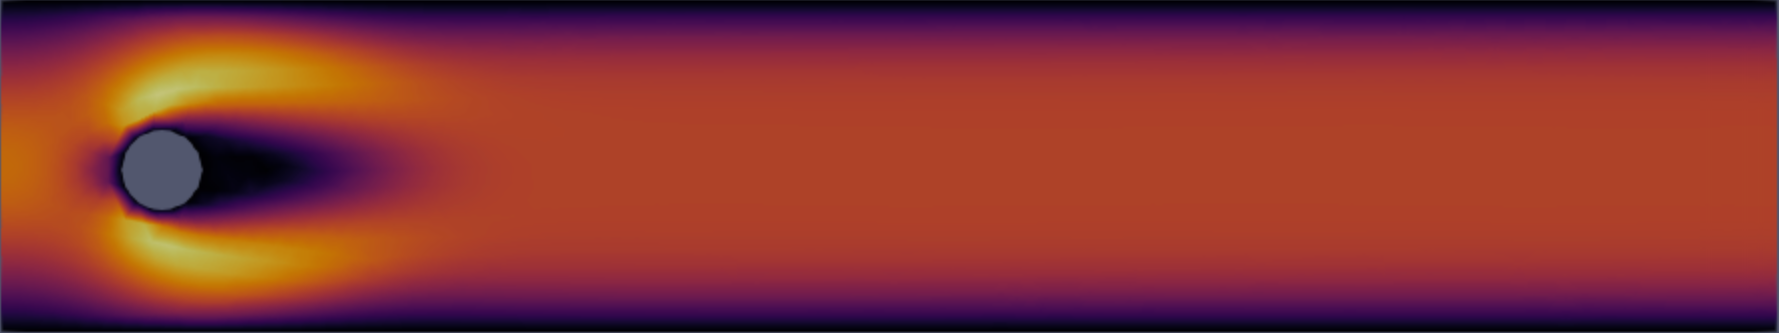
\includegraphics[width=.48\linewidth]{image/velocity-20-2d.png}\hfill
  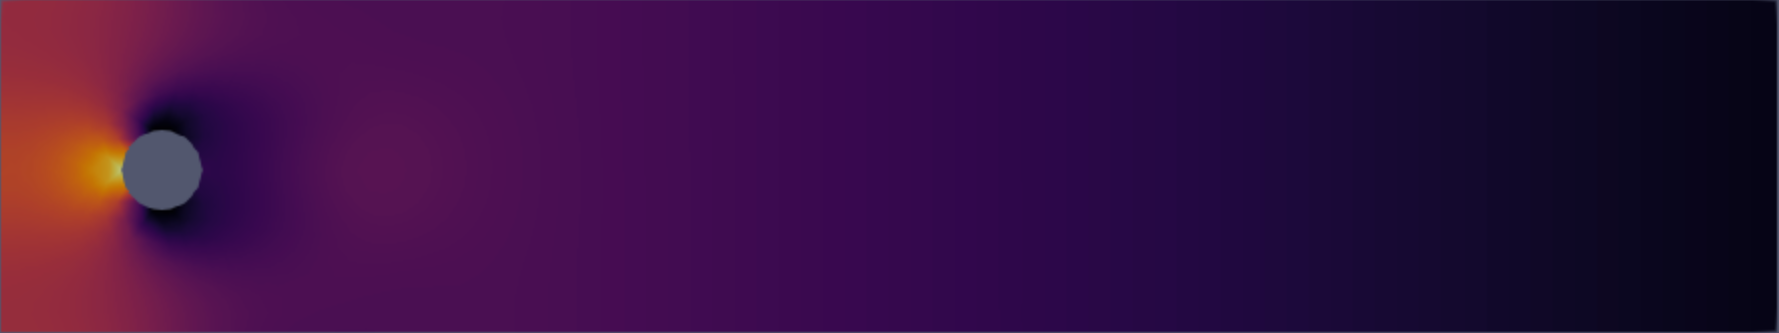
\includegraphics[width=.48\linewidth]{image/pressure-20-2d.png}\hfill
  \end{minipage}%
  \par
  \begin{minipage}{\linewidth}
  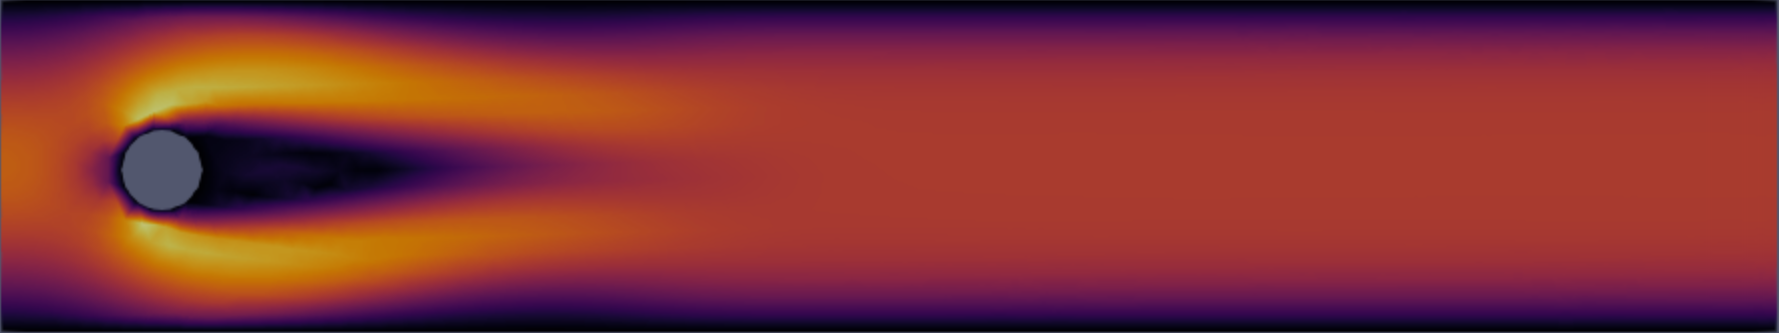
\includegraphics[width=.48\linewidth]{image/velocity-48-2d.png}\hfill
  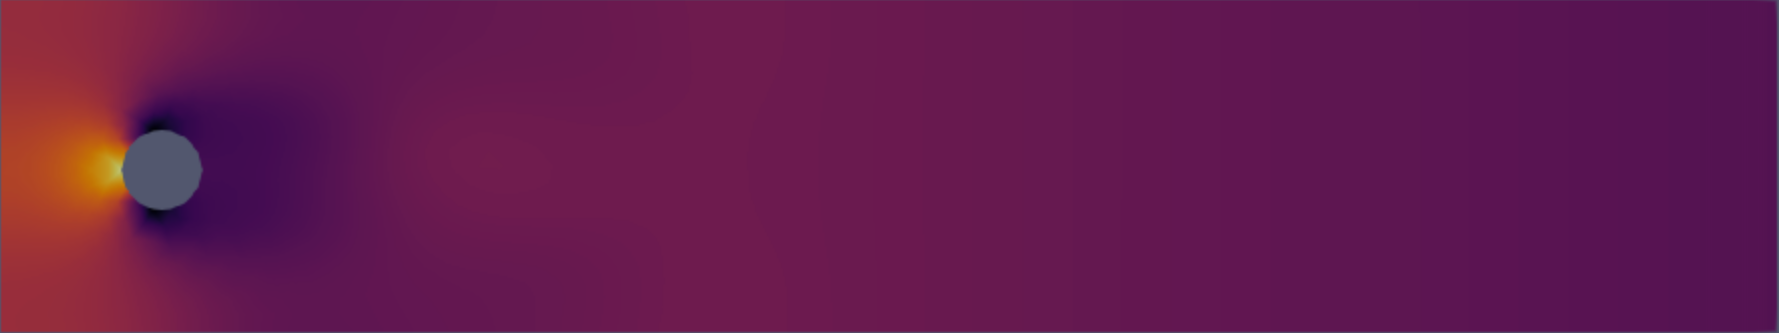
\includegraphics[width=.48\linewidth]{image/pressure-48-2d.png}\hfill
  \end{minipage}%
  \par
  \begin{minipage}{\linewidth}
  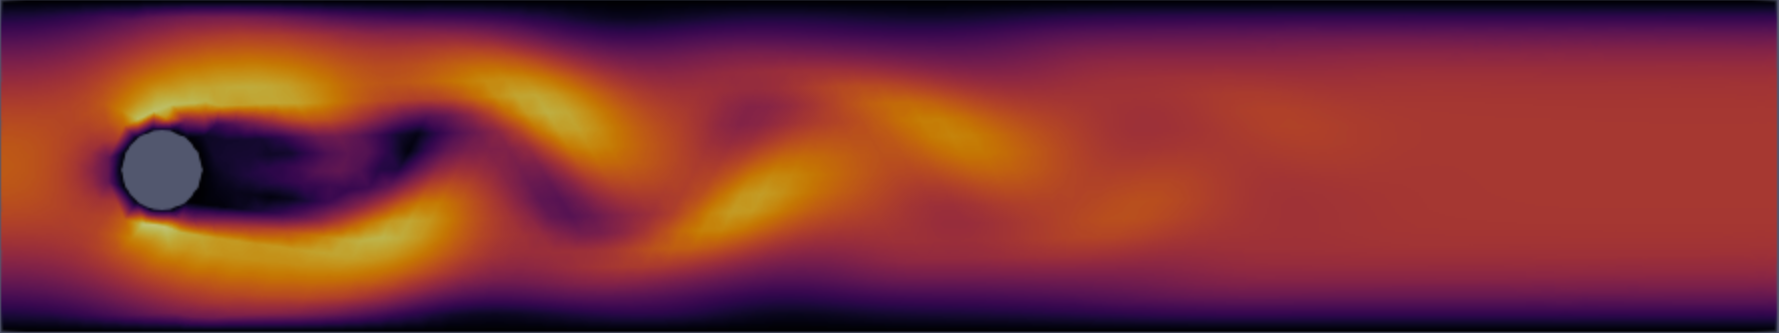
\includegraphics[width=.48\linewidth]{image/velocity-100-2d.png}\hfill
  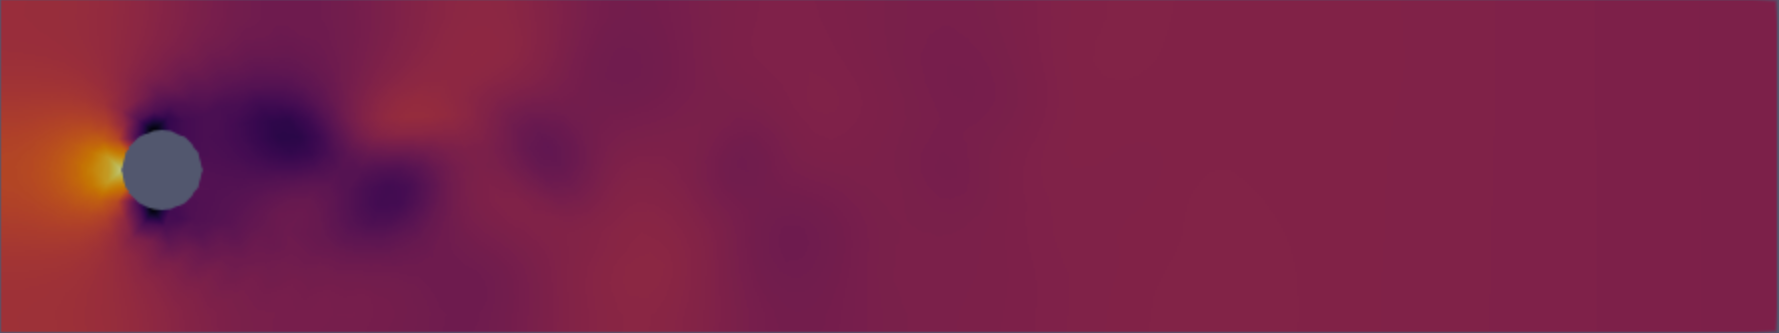
\includegraphics[width=.48\linewidth]{image/pressure-100-2d.png}\hfill
  \end{minipage}%
  \par
  \begin{minipage}{\linewidth}
  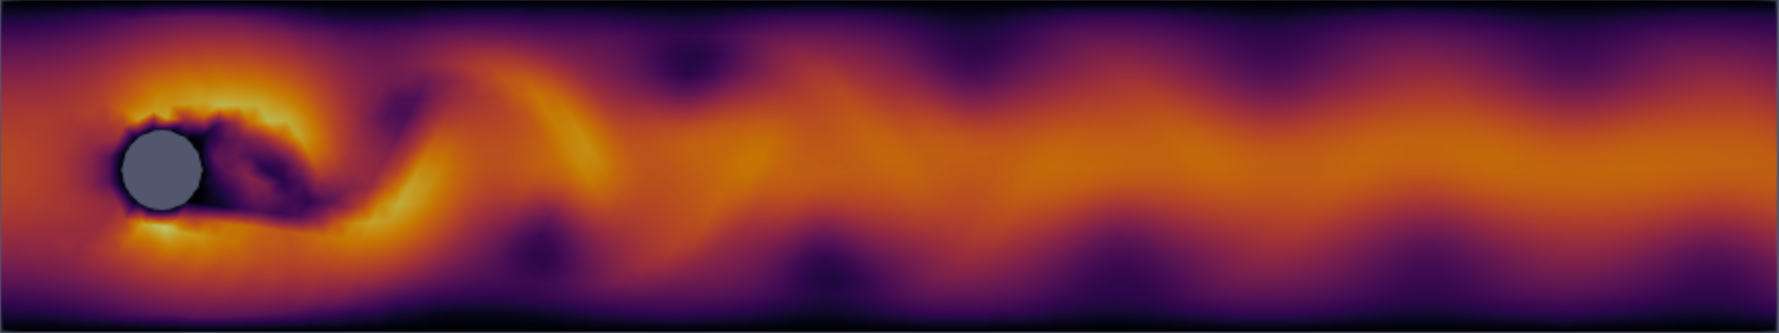
\includegraphics[width=.48\linewidth]{image/velocity-200-2d.png}\hfill
  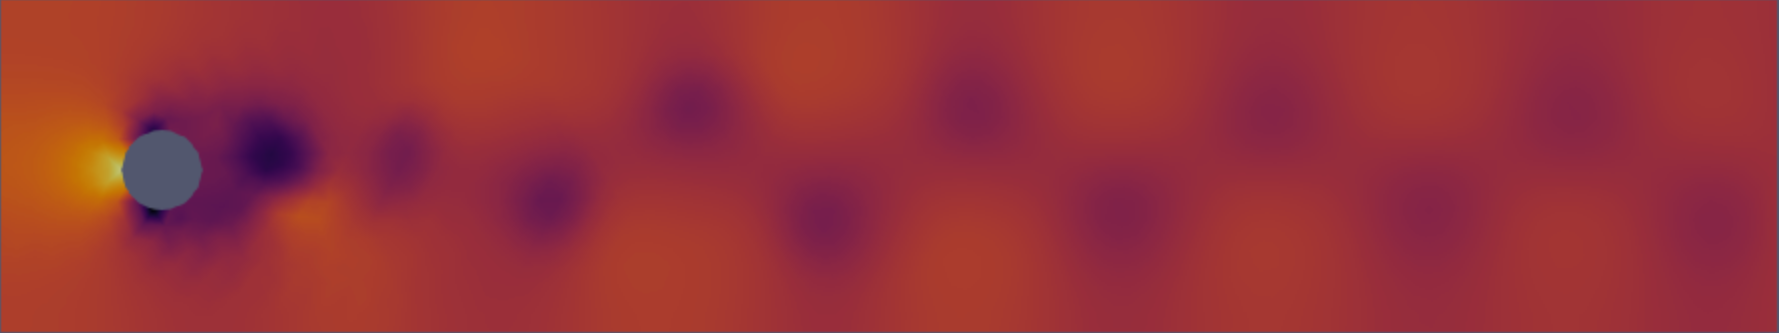
\includegraphics[width=.48\linewidth]{image/pressure-200-2d.png}\hfill
  \end{minipage}%
  
  \caption{Velocity (left) and pressure (right) at different levels of turbulence. The results were obtained with $\Delta t = 5 * 10^{-4}s$, on a mesh generated with the argument \texttt{-clmax 0.25} and are relative to $t = 1.35s$.}
  \label{fig:velocity-pressure-2d}
\end{figure}

\begin{figure}[h]
  \begin{minipage}{\linewidth}
  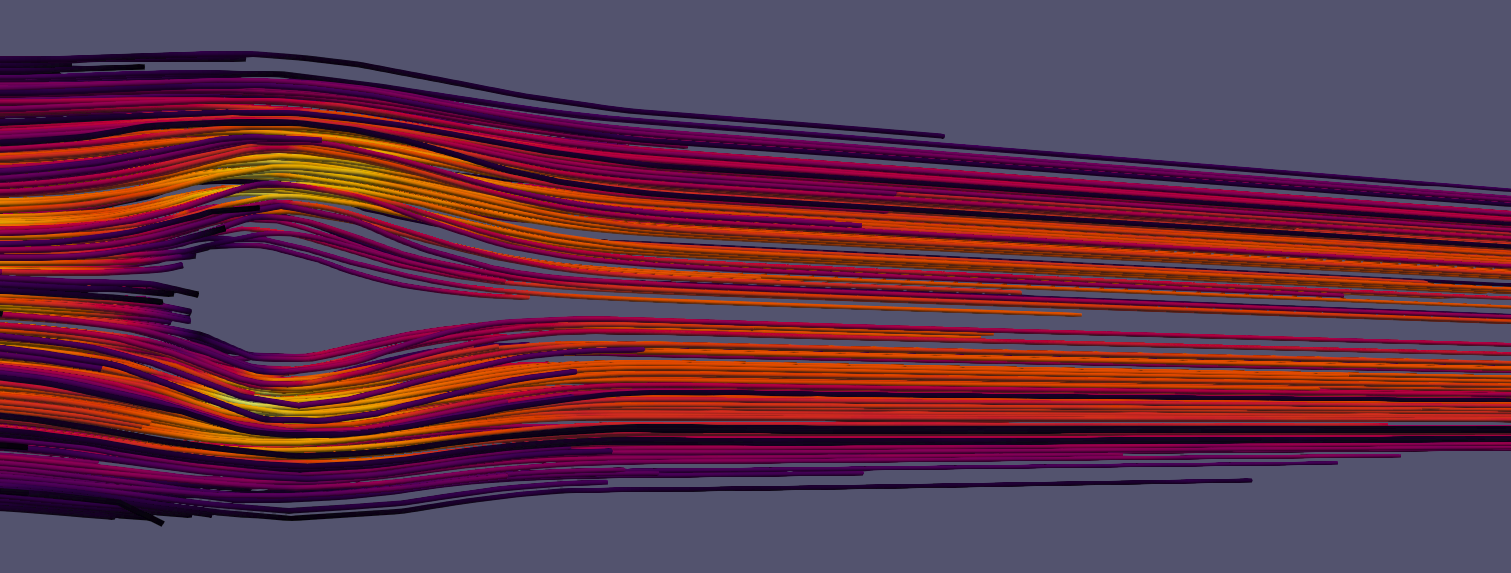
\includegraphics[width=\linewidth]{image/3d-arrows-20.png}\hfill
  \end{minipage}%
  \par
%   \begin{minipage}{\linewidth}
%   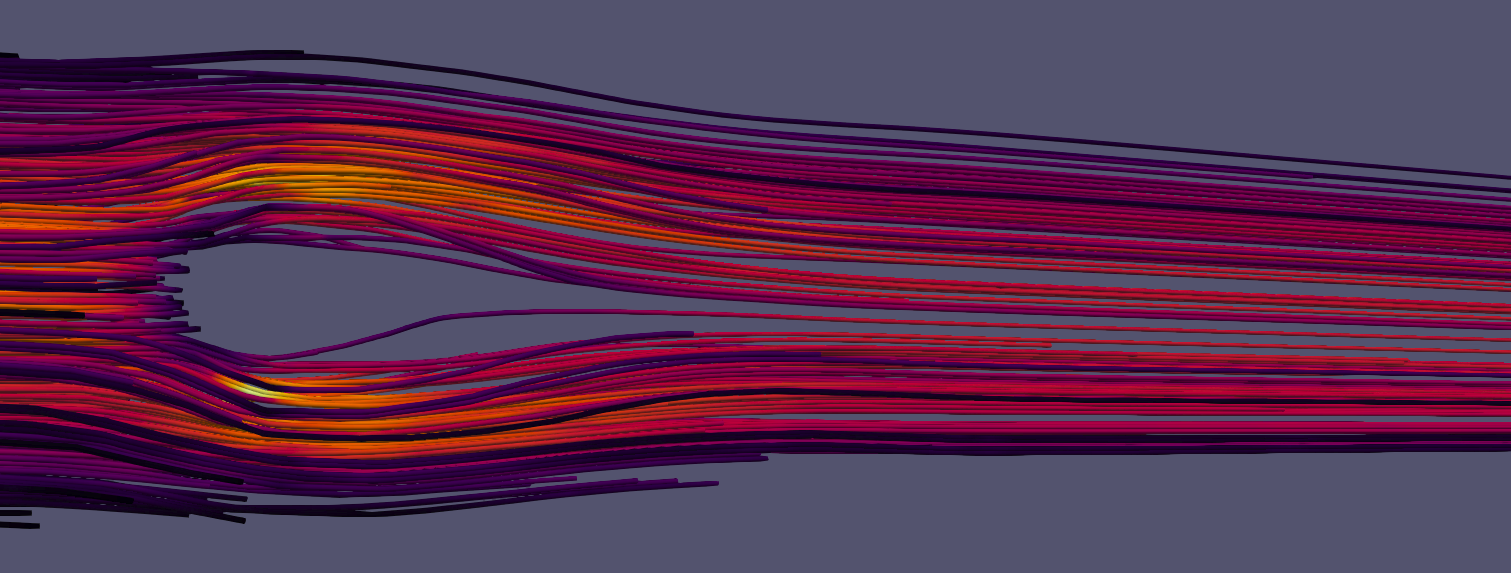
\includegraphics[width=\linewidth]{image/3d-arrows-48.png}\hfill
%   \end{minipage}%
%   \par
%   \begin{minipage}{\linewidth}
%   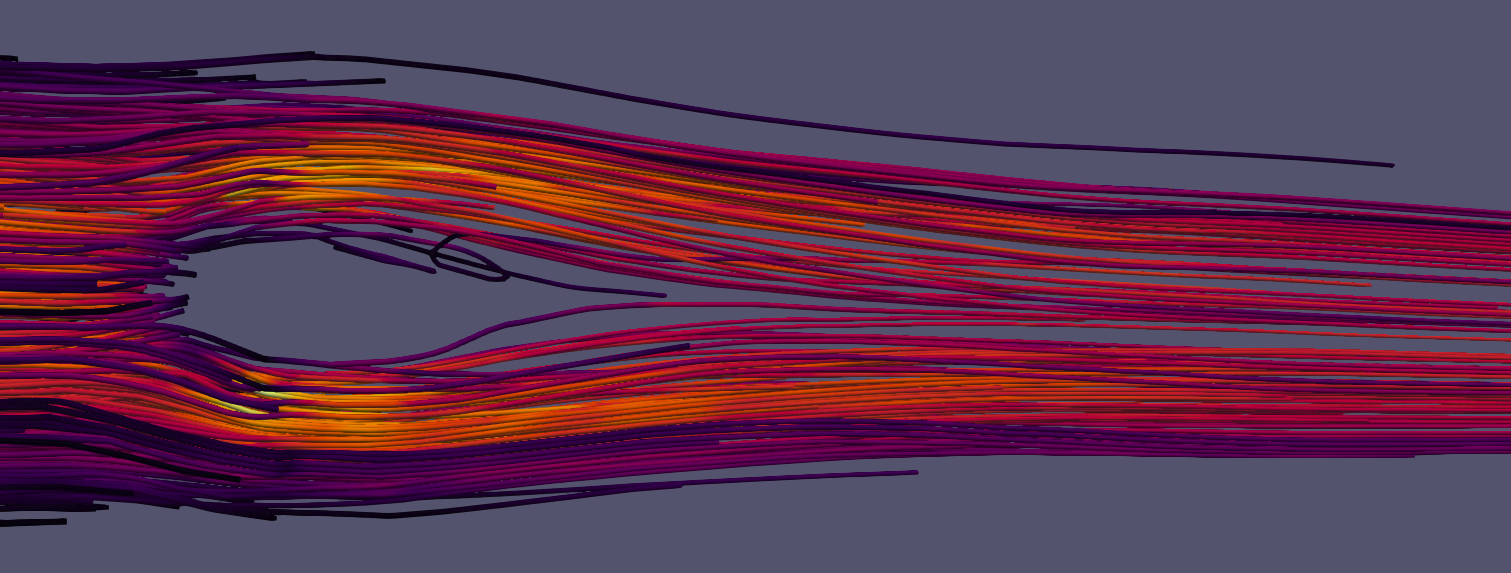
\includegraphics[width=\linewidth]{image/3d-arrows-100.png}\hfill
%   \end{minipage}%
%   \par
  \begin{minipage}{\linewidth}
  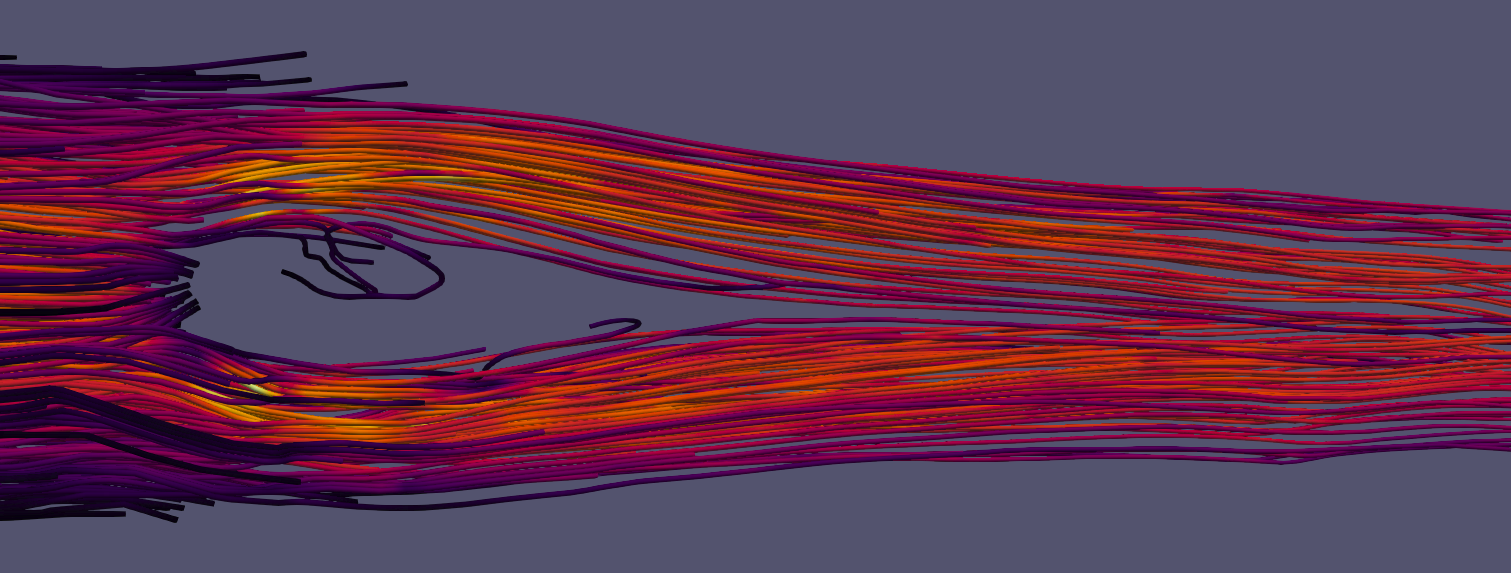
\includegraphics[width=\linewidth]{image/3d-arrows-200.png}\hfill
  \end{minipage}%
  
  \caption{Velocity stream lines at low and high Reynolds numbers, in 3D. The results were obtained with $\Delta t = 10^{-3}s$, on a mesh generated with the argument \texttt{-clmax 0.5} and are relative to $t = 1.5s$.}
  \label{fig:velocity-3d}
\end{figure}

\subsubsection{Results discussion}
A clear pattern can be seen in the velocity field, with the flow being laminar for low values of the Reynolds number and turbulent for higher values. This is consistent with the expected behavior of the flow, as vortex shedding is expected to occur for higher values of the Reynolds number. The pressure field is also consistent with the expected behavior, with the pressure being higher on the front of the cylinder and lower on the back.
The effects of vortex on lift and drag are also visible in section \ref{sec:lift_drag_plots}, where the lift and drag coefficients are plotted against time. 

\section{Lift and drag coefficients}
	\subsection{Background}
In laminar flow problems, the lift and drag coefficients play a crucial role in characterizing the aerodynamic behavior of an object in relative motion with a fluid. These coefficients are dimensionless parameters and are directly proportional to the lift and drag forces experienced by an object, and inversely proportional to the square of the reference relative velocity.

\subsubsection{Lift Coefficient}
The lift coefficient represents the efficiency of an airfoil or any aerodynamic shape in generating lift perpendicular to the direction of flow. In laminar flow, understanding the lift coefficient is essential for predicting the upward force that counters the weight of an object (e.g., an aircraft wing).
\subsubsection{Drag Coefficient}
The drag coefficient characterizes the resistance an object experiences parallel to the flow direction. In laminar flow, it is critical for estimating the drag force opposing the object's motion through the fluid.
    
\subsection{Calculation}
\subsubsection{Equations in the benchmark}
According to the definitions given in the suggested paper \cite{Cylinder}, the lift and drag forces are:
\begin{equation}
F_L = - \int_S (\rho \nu \frac{\partial v_t}{\partial n}n_x + P n_y) \, dS
\end{equation}
\begin{equation}
F_D = \int_S (\rho \nu \frac{\partial v_t}{\partial n}n_y - P n_x) \, dS
\end{equation}
With the following notation: $\mathcal{S}$ (a circular curve in two dimensions, and a capless cylinder's surface in three dimensions), normal vector $\mathbf{n}$ on $\mathcal{S}$ with x-component $n_x$ and y-component $n_y$, tangential velocity $v_t$ on $\mathcal{S}$, pressure $P$ and tangent vector $\mathbf{t} = (n_y, -n_x)$ or $\mathbf{t} = (n_y, -n_x, 0)$, depending on the problem's dimensionality.

After calculating the lift and drag forces, the corresponding lift and drag coefficients are, in the two dimensional case:
\begin{equation}\label{eq:lift_coeff}
    C_L = \frac{2F_a}{\rho \bar{U}^2 D}
\end{equation}
\begin{equation}\label{eq:drag_coeff}
    C_D = \frac{2F_w}{\rho \bar{U}^2 D}
\end{equation}
While in the three dimensional case the equations have an additional $H$ factor in the denominator.

\subsubsection{Issues with the equations}
These definitions suffer from multiple issues: for example, the terms $F_w$ and $F_a$ are never defined in \cite{Cylinder} and the formulae do not match with the ones given in the project description, not even in terms of physical units of measurement. As such, we compared multiple sources in the scientific literature and decided to use the formulae supported by the largest number of reliable sources. 

\paragraph{Lift and drag forces}
Regarding the computation of the lift and drag coefficients utilizing the computed forces, both \cite{Dede} and \cite{lift_drag} provide the same formula as Equation \ref{eq:drag_coeff}, where $F_w$ is the drag force.  For this reason, we decided to use Equations \ref{eq:lift_coeff} and \ref{eq:drag_coeff} and their 3D generalization, using $F_L$ and $F_D$ in place of $F_a$ and $F_w$.

\paragraph{Lift and drag coefficients}
Regarding the calculation of the drag and lift forces, we decided to use the formula for the drag force presented by \cite{Dede}. Said formula is similar to the one used in \cite{lift_drag}, which we used to generalize it to the lift force computation. The formulae we used for both the two and three dimensional cases are therefore:
\begin{equation}\label{eq:lift_force}
    F_L = \int_S \rho ((\nu (\nabla u + \nabla u^T) - p I)\mathbf{n}) \cdot \hat{j} dS
\end{equation}
\begin{equation}\label{eq:drag_force}
    F_D = \int_S \rho ((\nu (\nabla u + \nabla u^T) - p I)\mathbf{n}) \cdot \hat{i} dS
\end{equation}
Where $I$ is the identity tensor, $\hat{i}$ and $\hat{j}$ are the unit vectors in the $x$ and $y$ direction respectively and $\mathbf{n}$ has the same meaning as in the previous equations. The notation in \cite{Dede} and \cite{lift_drag} was not adopted, as to match the notation used in the rest of the report.

\subsubsection{More accurate equations}
The described formulae suffer from one more issue: since we are integrating terms depending on the pressure and on the gradient of the velocity over a boundary with one less physical dimension that $\Omega$, the operation is not well-defined in the weak sense.

\paragraph{New equations}
A method to compute the drag coefficient in two dimensions in a well-defined manner that gives enhanced precision is provided in \cite{Dede}, which we extended to the computation of the lift coefficient and to the three dimensional case. In particular, this method consists in finding two functions $\mathbf{\phi}_\infty^L$ and $\mathbf{\phi}_\infty^D$ in $(H^1(\Omega))^d$ that satisfy the following constraints:
\begin{equation}\label{eq:phi_inf_lift}
    \mathbf{\phi}_\infty^L|_{\mathcal{S}} = -\hat{j} \land \mathbf{\phi}_\infty^L|_{\partial\Omega \setminus \mathcal{S}} = \mathbf{0}
\end{equation}
\begin{equation}\label{eq:phi_inf_drag}
    \mathbf{\phi}_\infty^D|_{\mathcal{S}} = -\hat{i} \land \mathbf{\phi}_\infty^D|_{\partial\Omega \setminus \mathcal{S}} = \mathbf{0}
\end{equation}
And then letting 
\begin{equation}\label{eq:force_weak}
    F = \int_{\Omega} \nu \nabla \mathbf{u} : \nabla \mathbf{\mathbf{\phi}_\infty} \, d\Omega + \int_{\Omega} ((\mathbf{u} \cdot \nabla) \mathbf{u}) \cdot \mathbf{\phi}_\infty \, d\Omega - \int_{\Omega} p \nabla \cdot \mathbf{\phi}_\infty \, d\Omega
\end{equation}
Where $F$ and $\mathbf{\phi}_\infty$ are $F_L$ or $F_D$ and $\mathbf{\phi}_\infty^L$ or $\mathbf{\phi}_\infty^D$ for the lift and the drag forces respectively. 

\paragraph{Discretization}
We then discretized the equation in space, using the same finite element space as for the discrete problem, and looked for two functions $\mathbf{\phi}_{\infty h}^L$ and $\mathbf{\phi}_{\infty h}^D$ which fit Equations \ref{eq:phi_inf_lift} or \label{phi_inf_drag} for all test functions $\mathbf{v}_h$ in $V_h$. Since there are infinitely many functions that meet the conditions, we set the additional constraint:
\begin{equation}
    \int_\Omega \mathbf{\phi}_\infty \mathbf{v}_h \, d\Omega = 0 \; \forall \mathbf{v}_h \in V_h
\end{equation}
Which results in linear systems that can be solved using the already assembled and relatively well-conditioned mass matrix for the velocity and using the lifting technique.

\subsection{Results}\label{sec:lift_drag_plots}
Figure \ref{fig:lift-drag} shows the plot of the lift and drag coefficients over time for the two and three dimensional flow past a cylinder benchmark and multiple values of Reynolds number. 2D results use $\Delta t = 5*10^{-4}s$ and \texttt{-clmax 0.25}, while 3D results use $\Delta t = 10^{-3}s$ and \texttt{-clmax 0.5}. The result for $t = \Delta t$ was removed from the images, as it is out of scale due to the sudden change in the inlet velocity. The black line reports the results obtained with Formulae \ref{eq:lift_force} and \ref{eq:drag_force}, while the red line reports the results obtained with Formula \ref{eq:force_weak}. 3D simulations were run before the implementation of the new formula for calculation of the forces.

\begin{figure}[]
    \centering
    \subfigure[2D problem, Re = 48]{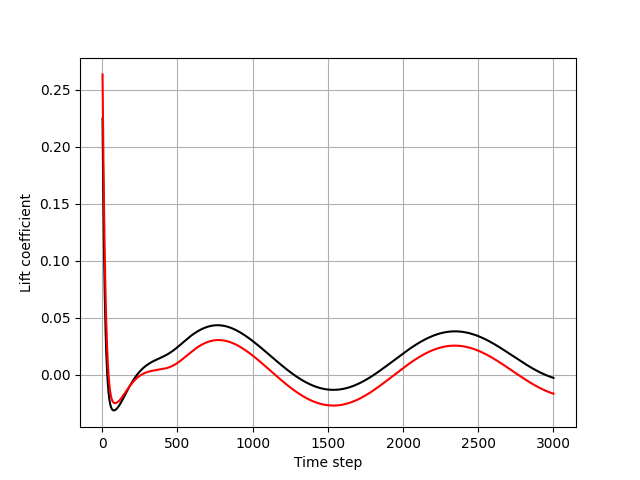
\includegraphics[width=38mm]{image/2d-lift-48}}
    \subfigure[2D problem, Re = 48]{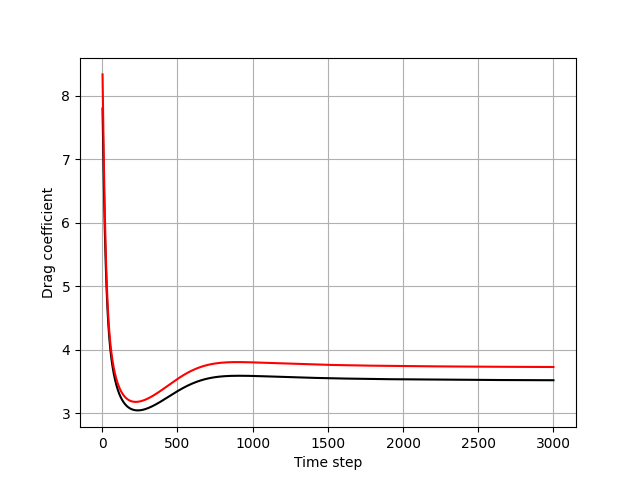
\includegraphics[width=38mm]{image/2d-drag-48}}
    \subfigure[2D problem, Re = 200]{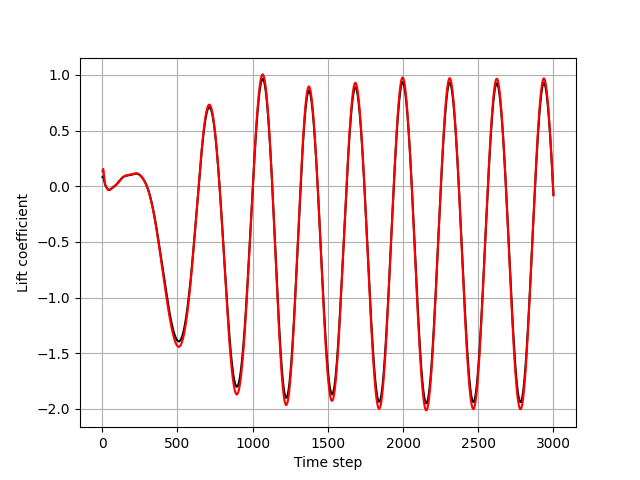
\includegraphics[width=38mm]{image/2d-lift-200}}
    
    \subfigure[2D problem, Re = 200]{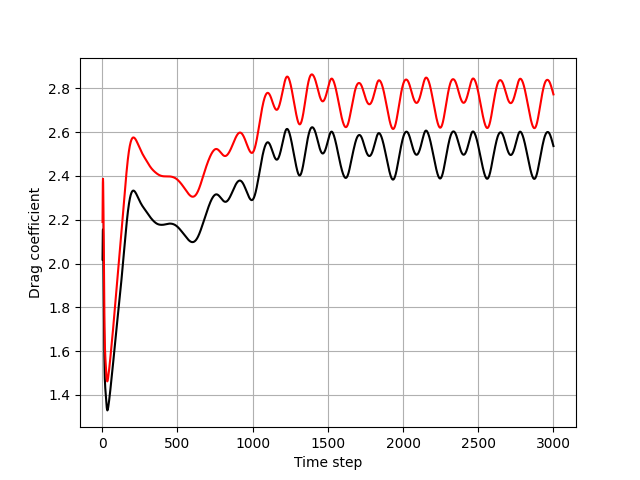
\includegraphics[width=38mm]{image/2d-drag-200}}
    \subfigure[3D problem, Re = 133]{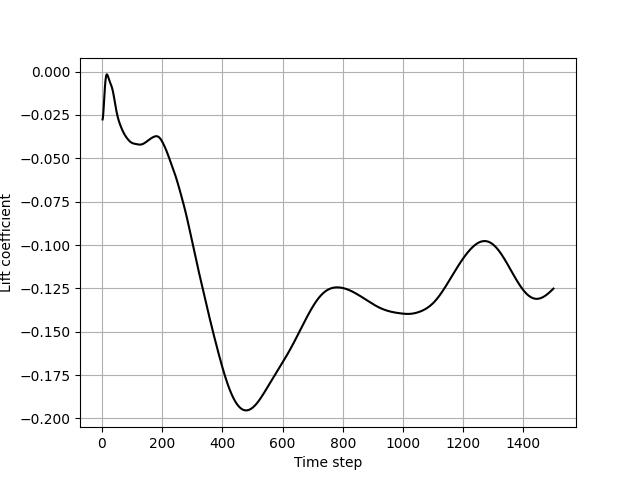
\includegraphics[width=38mm]{image/3d-lift-3.0}}
    \subfigure[3D problem, Re = 133]{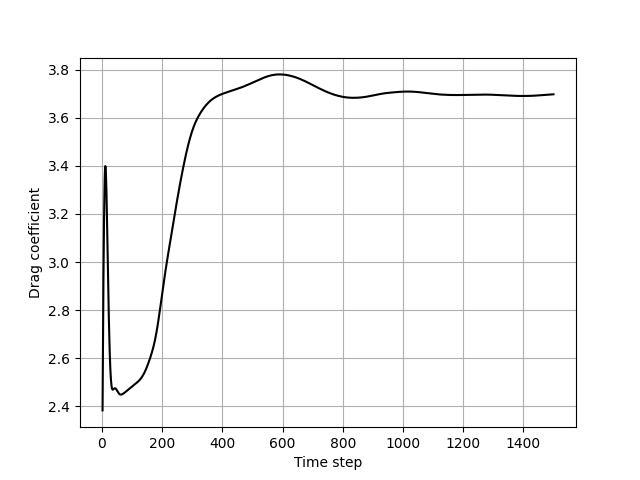
\includegraphics[width=38mm]{image/3d-drag-3.0}}
    
    \caption{Plot of lift and drag coefficients over time for the test case with constant inlet velocity. On the $x$ axis, the time step $n$ is reported, where $t = n\Delta t$.}
    \label{fig:lift-drag}
\end{figure}

\subsection{Results discussion}
While we were unable to find results for our exact test, multiple sources in the scientific literature show a qualitative behaviour of the lift and drag coefficients similar to ours for similar problems \cite{lift_drag}\cite{lift_drag_2}\cite{lift_drag_3}. Namely, the lift coefficient oscillates over time, with a frequency that increases with the Reynolds number, while the drag coefficient starts at a high value, decreases to a minimum and then increases again, with small oscillations for Re = 200.

We tested other configurations of Reynolds numbers, both in 2D and 3D, but did not include the results for the sake of brevity. Regarding the test case with a time dependent inlet velocity, in this test case the Reynolds number is a sine wave with semiperiod $8s$. As expected, when the time tends to $0$ or to $8s$, the absolute value of the drag coefficient tends to infinity, as it is inversely proportional to the Reynolds number for small values of Re. 

\section{Preconditioners}\label{sec:preconditioners}
	\subsection{Implemented preconditioners}
To solve the linear systems arising from the discretization of the Navier-Stokes equations, a variety of preconditioners have been implemented. The preconditioners are based on the ones presented in \cite{Quarteroni} and are the following ones:
\begin{itemize}
    \item Block diagonal preconditioner
    \item SIMPLE preconditioner
    \item aSIMPLE preconditioner
    \item Yoshida preconditioner
\end{itemize}
The diagonal preconditioner was adapted from the code in laboratory 9 and used during development of the other preconditioners and for comparison. 

\paragraph{SIMPLE}
The \texttt{SIMPLE} preconditioner is defined as:
\begin{equation}
    P_{SIMPLE} = \begin{bmatrix}
        F & 0 \\
        B & -\tilde{S} 
    \end{bmatrix}
    \begin{bmatrix}
        I & D^{-1}B^T \\
        0 & \alpha I
    \end{bmatrix}
\end{equation}
Where $D$ is the diagonal of $F$ and $\alpha$ is a parameter that can be tuned to damp the pressure update. The value $\tilde S$ is an approximation of the Schur complement, and is defined as:

\begin{equation}
    \tilde{S} = B D^{-1} B^T
\end{equation}

\paragraph{aSIMPLE}
The \texttt{aSIMPLE} (approximate SIMPLE) preconditioner is a modified version of the \texttt{SIMPLE} preconditioner, and its inverse can be computed directly as:
\begin{equation}
    \begin{split}
        & P_{aSIMPLE}^{-1} = \\
        & \begin{bmatrix}
            D^{-1} & 0 \\
            0 & I
        \end{bmatrix}
        \begin{bmatrix}
            I & -B^T \\
            0 & I
        \end{bmatrix}
        \begin{bmatrix}
            D & 0 \\
            0 & \dfrac{1}{\alpha}I
        \end{bmatrix} 
        \begin{bmatrix}
            I & 0 \\
            0 & -\hat{\tilde{S}}^{-1}
        \end{bmatrix}
        \begin{bmatrix}
            I & 0 \\
            -B & I
        \end{bmatrix}
        \begin{bmatrix}
            \hat{F}^{-1} & 0 \\
            0 & I
        \end{bmatrix}
    \end{split}
\end{equation}
Where $\hat{F} \approx F$ and $\hat{\tilde{S}} \approx \tilde{S}$.

\paragraph{Yoshida}
The \texttt{Yoshida} preconditioner is based on the Yoshida's method. The preconditioner is defined as:
\begin{equation}
    P_{Yoshida} = \begin{bmatrix}
        F & 0 \\
        B & -\Delta t B M^{-1} B^T 
    \end{bmatrix}
    \begin{bmatrix}
        I & F^{-1} B^T \\
        0 & I
    \end{bmatrix}
\end{equation}
Once again, the term $\Delta t B M^{-1} B^T$ is an approximation of the Schur complement. The actual implementation of the preconditioner approximates $M$ with its diagonal.

\subsection{Implementation details}
Clearly, preconditioners were implemented using their structure as the product of block diagonal or block triangular systems. 

The approximations of the Schur complements were computed explicitly and diagonal matrices were inverted, while terms requiring the resolution of linear systems on $F$, $\tilde{S}$ or $\Delta t B M^{-1} B^T$ were solved using GMRES as an iterative solver with an appropriate preconditioner. Namely, the supported preconditioners are the algebraic multigrid and ILU preconditioners implemented in \texttt{Trilinos\-Wrappers::\-PreconditionAMG} and \texttt{Trilinos\-Wrappers::\-PreconditionILU} respectively. This choice can be made setting the flag \texttt{-l}.

Regarding the terms $\hat{F}$ and $\hat{\tilde{S}}$ in \texttt{aSIMPLE}, we support both the same approach used for $F$ and $\tilde{S}$, i.e. solving the linear system with GMRES, and setting $\hat{F}$ and $\hat{\tilde{S}}$ to their algebraic multigrid or ILU preconditioners. The choice between the two options can be made by setting the flag $\texttt{-i}$.

\subsection{Performance}
As stated in \cite{Quarteroni}, all implemented preconditioners require the choice of a relatively small value for $\Delta t$, as their approximations of the Schur complement deteriorate when $\Delta t$ increases.

While we took performance into consideration in the whole codebase, avoiding expensive operations and serial bottlenecks aside from the mesh initialization, the linear system resolution code is the only part whose performance was analyzed quantitatively.

Table \ref{tab:performance} shows performance results for the preconditioners, on the three dimensional flow past a cylinder problem and with multiple inner preconditioners. The results are relative to $\Delta t = 10^{-3}$ and \texttt{-clmax 0.05} and were obtained using the MOX cluster and 10 MPI processes. The tolerance for the outer and inner solvers was $10^{-7}$ and $10^{-5}$ respectively, and $\alpha$ was set to $1$. These values were chosen as they were experimentally a sweet spot between performance and result precision. In particular, reducing the precision of the inner solver has an experimentally small impact on performance, but it can create issues with precision. Results were obtained using \texttt{chrono} and include both the time for building the preconditioner and the time to solve the linear system.

Table \ref{tab:scaling} shows performance results for \texttt{aSIMPLE} with no inner solver and the AMG preconditioner with multiple numbers of MPI processes.

\begin{table}[h]
    \centering
    \begin{tabular}{P{30mm}|P{17mm}|P{17mm}|P{17mm}|P{17mm}}
        Preconditioner & Time (AMG) & Iterations (AMG) & Time (ILU) & Iterations (ILU)\\
        \hline
        \texttt{Block diagonal} & - & - & - & -\\
        \texttt{SIMPLE} & 4.0s & 39 & 3.5s & 37\\
        \texttt{aSIMPLE} & 4.2s & 32 & 3.9s & 37\\
        \texttt{aSIMPLE -i} & 1.4s & 137 & - & -\\
        \texttt{Yoshida} & 7.4s & 37 & 6.7s & 39\\
    \end{tabular}
    \caption{Execution times and GMRES iterations for each preconditioner on the first iteration of the 3D flow past a cylinder problem. \texttt{aSIMPLE -i} refers to the preconditioner \texttt{aSIMPLE} without the usage of an inner solver. The symbol - means no convergence in 10000 iterations.}
    \label{tab:performance}
\end{table}

\begin{table}[h]
    \centering
    \begin{tabular}{c|c|c}
        Processes & Time & Iterations\\
        \hline
        1 & 10.2s & 178\\
        5 & 2.3s & 160\\
        10 & 1.4s & 137\\
        15 & 1.7s & 159\\
        20 & 1.8s & 161\\
    \end{tabular}
    \caption{Execution times and GMRES iterations with multiple numbers of MPI processes for \texttt{aSIMPLE} with no inner solver and using the AMG preconditioner.}
    \label{tab:scaling}
\end{table}

\subsubsection{Results discussion}
The data presented in Table \ref{tab:performance} and from other tests shows the following findings:
\begin{itemize}
    \item While the block diagonal preconditioner performs sufficiently well to be used for coarse meshes and as a tool to aid development, it is unsuitable for Navier-Stokes problems with fine meshes and the need for better performing preconditioners is evident.
    \item When inner solvers are used, the preconditioners \texttt{SIMPLE} and \texttt{aSIMPLE} perform similarly and better than \texttt{Yoshida}. Moreover, ILU performs slightly better than AMG as a preconditioner for the inner solvers.
    \item The \texttt{aSIMPLE} preconditioner with no inner solver is by far the best performing, despite the larger number of GMRES iterations, as each iteration is by far less computationally demanding. This result matches with the results presented in \cite{Quarteroni}. The ILU preconditioner is not suitable in this case, showing that the matrices are better approximated by their AMG preconditioner than by their incomplete LU factorizations.
\end{itemize}
Regarding the best performing preconditioner, \texttt{aSIMPLE} with no inner solver, the results are as follows:
\begin{itemize}
    \item As shown in Table \ref{tab:scaling}, the preconditioner scales well up to around 10 cores, achieving a $7.3x$ speed-up over the serial computation. After that amount, testing with up to 20 processes, the preconditioner appears to be scalable in the sense that the number of GMRES iterations does not increase. However, when using more than 10 processes, execution time does not decrease, instead increasing slightly. This shows that either the parallelism expressed by the solver is exhausted by 10 processes or that there is another bottleneck, which might be the memory access time or the overhead for communication. While \cite{Quarteroni} presents much better scaling with the number of cores, this is likely due to the fact that more complex and better performing approximations $\hat{F} \approx F$ and $\hat{\tilde{S}} \approx \tilde{S}$ are used in said work.
    \item Further tests with \texttt{-clmax} ranging from 0.5 to 0.05 show that the preconditioner is experimentally optimal, as the number of GMRES iterations does not increase with the matrix dimension, remaining in the range $[150, 210]$ for 4 MPI processes. In particular, the number of iterations for \texttt{-clmax 0.05} is lower than with multiple coarser meshes.
\end{itemize} 

\section{Conclusions}
    In conclusion, we implemented and tested a solver for the incompressible and unsteady Navier-Stokes equations, supporting a variety of physical problems. We then applied the solver to the two and three dimensional flow past a cylinder benchmark, computing the velocity, pressure and lift and drag coefficients for a variety of configurations and commenting on the results. Finally, we implemented multiple preconditioners for the problem and analyzed the performance, scalability and optimality of the best performing one.

\bibliographystyle{unsrt}
\bibliography{bibliography}

\end{document}